\chapter{Block Controller Board}

This chapter presents two block controller boards, a quad block controller and a combo block controller board. While not every layout will favor a quad block controller, scaling the design down to two or even one block is rather straightforward. The combo block controller offers two blocks or one block with a higher amperage. 

\section{Block Diagram}

The following schematics show the block controller board for the quad block version. First, there is the main controller part with the connectors, the Raspberry PI PICO, the non-volatile memory, the CAN Bus line driver and the level shifters for the external connector pins used. Note that all the digital pins DIO0 to DIO7 are not exported, they are used on the board itself. The block controller also make use of the track lane connector, which routes the track power signals from the block controller board to the extension board. This way, no extra cables need to be wired from block controller to extension board for this purpose. The connector features four track channels, each for a nominal amperage of 3 Amps. This version of the block controller sends the first block track power on channel 1 and 2 and the second block track power on channel 3 and 4. Depending on future designs, the channel could be combined for a higher amperage or kept separate for up to four blocks.

\begin{figure}[htbp]
    \centering
    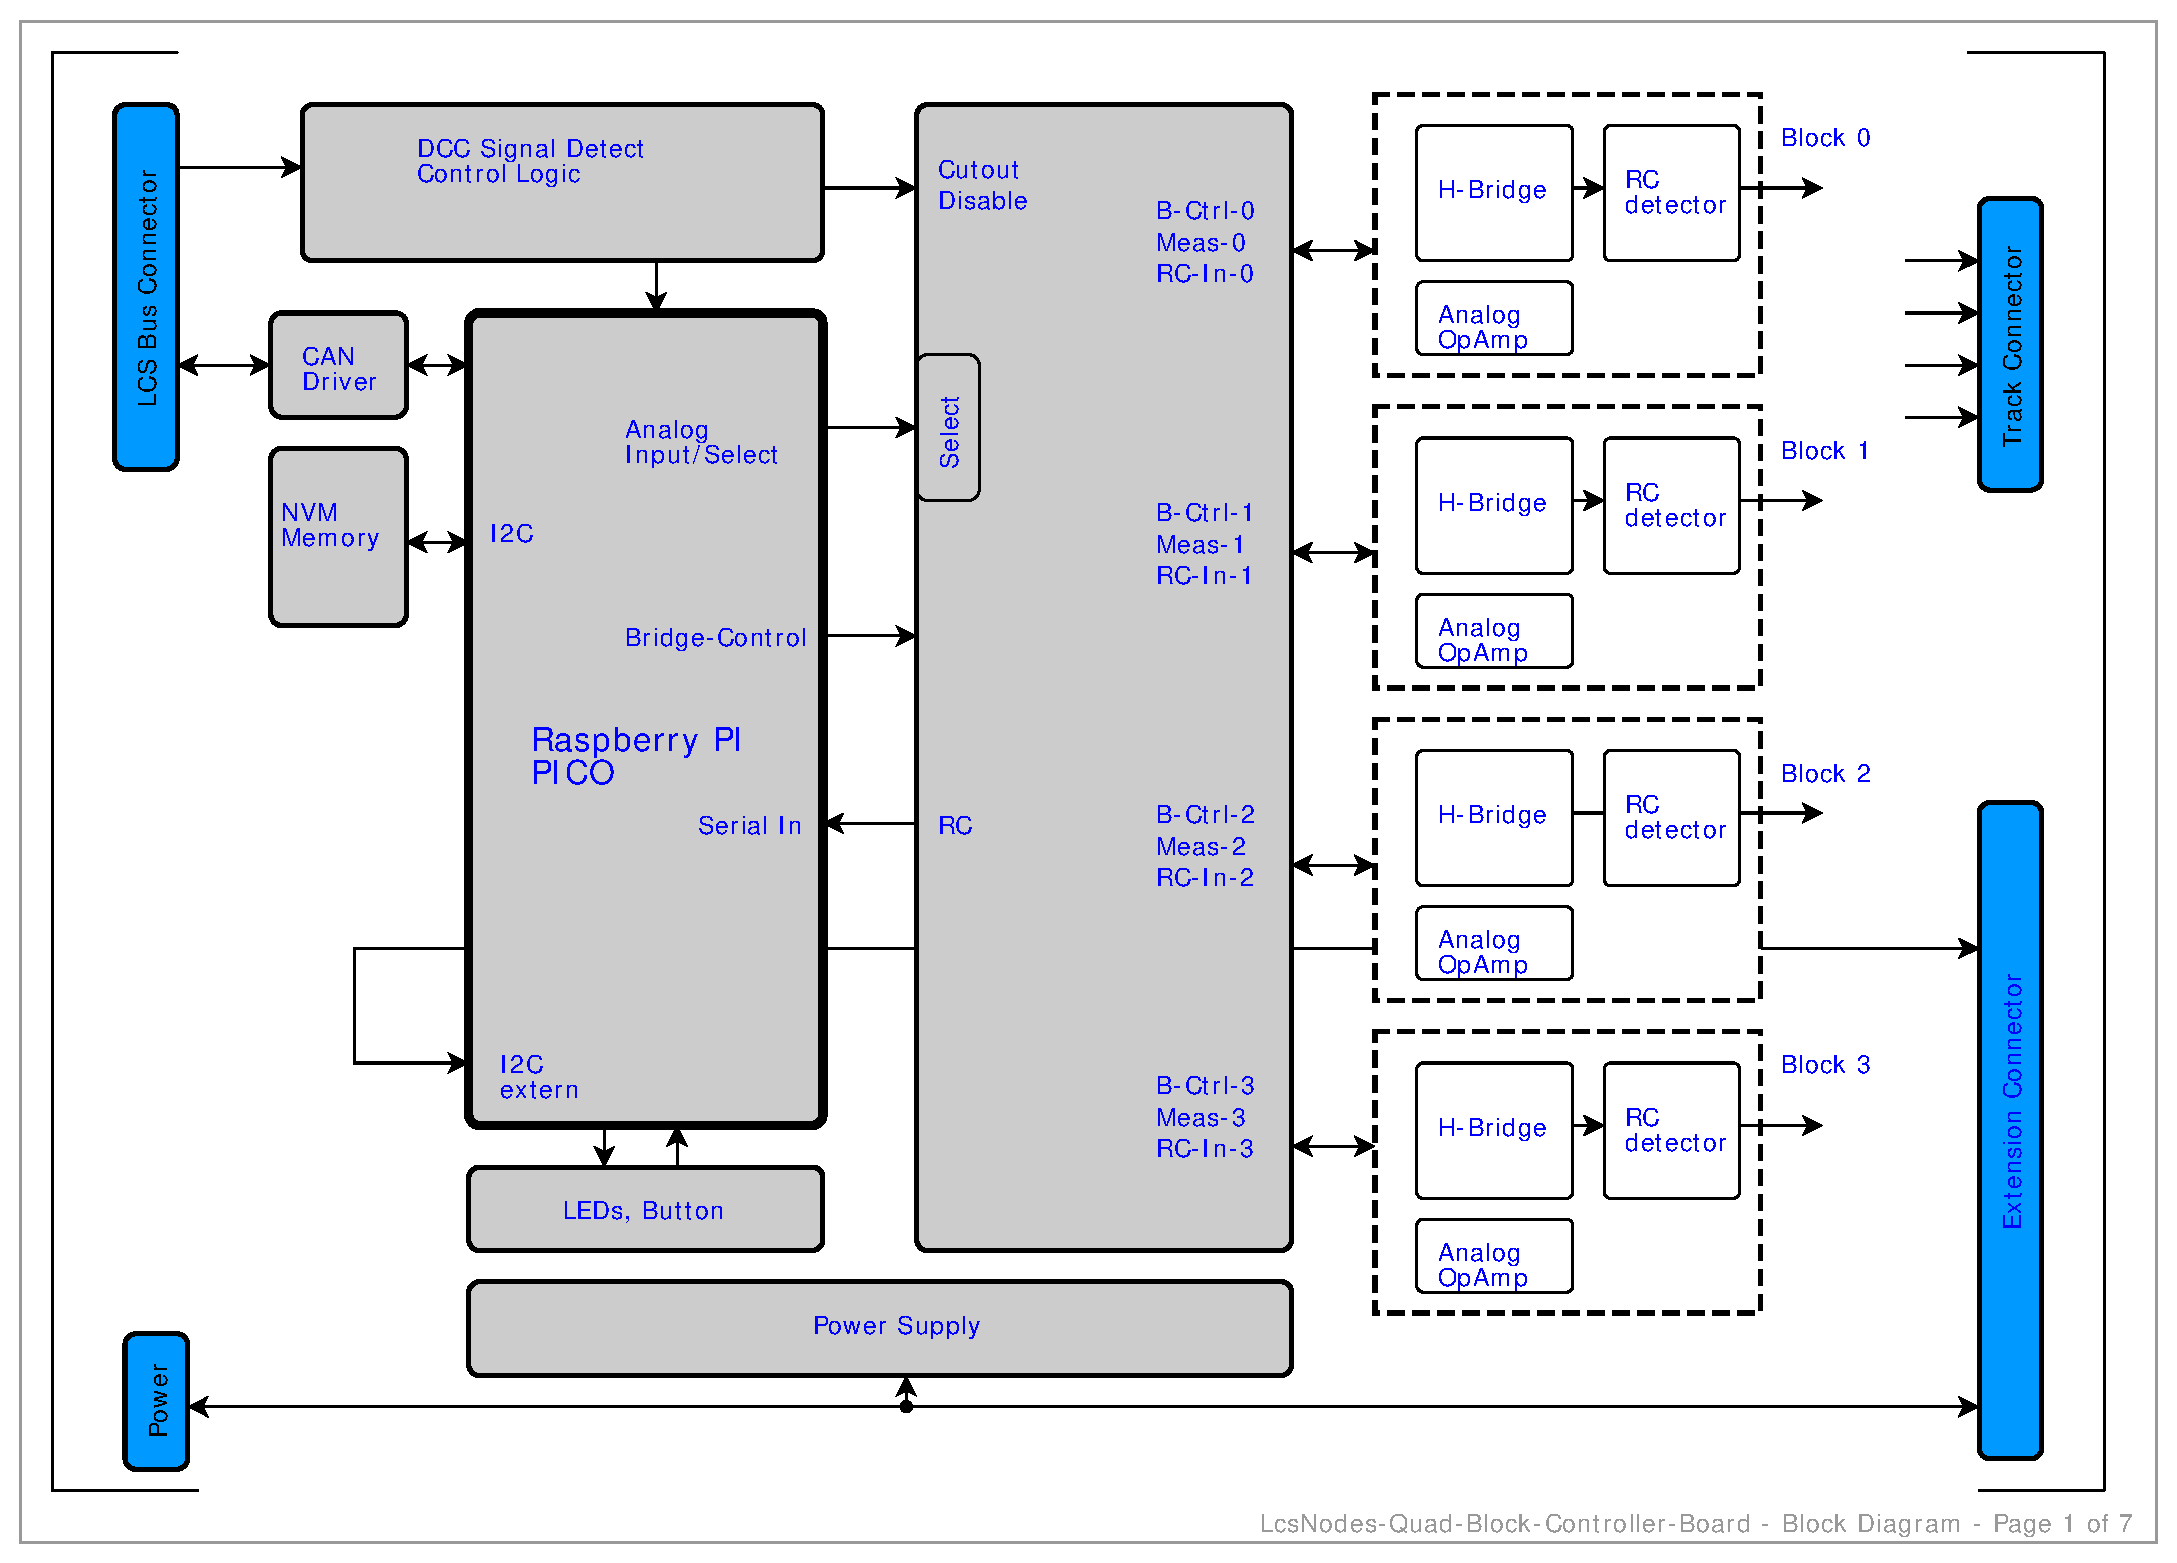
\includegraphics[page=1, width=0.6\textwidth]{./Schematics/Schematic_LcsNodes-Block-Quad-Controller.pdf}
    %\label{fig:schematic}
\end{figure}
\FloatBarrier

\section{Controller}

The first schematic shows the main controller Raspberry PI Pico, the level shifters required for the extension connector pins, the CAN bus driver and the non-volatile memory. This part is very similar to the main controller board shown in the previous chapters.

\begin{figure}[htbp]
    \centering
    \includegraphics[page=2, width=0.7\textwidth]{./Schematics/Schematic_LcsNodes-Block-Quad-Controller.pdf}
    %\label{fig:schematic}
\end{figure}
\FloatBarrier

\section{H-Bridge Decoding Logic}

There are four command to control the H-bridge. All decoding logic for the power unit control is done with dual 4-1 selectors. The signal from the opto-coupler is actually inverted, the wires need to be crossed for DCC signal input. All other signals are active high signals. 

\begin{figure}[htbp]
    \centering
    \includegraphics[page=3, width=0.7\textwidth]{./Schematics/Schematic_LcsNodes-Block-Quad-Controller.pdf}
    %\label{fig:schematic}
\end{figure}
\FloatBarrier

The bridge overall state, i.e. whether active or disconnected is controlled by an OR/AND gate, which will disable the bridge when both control signals are zero. For PWM mode, one side of the bridge will be at the zero level while the other will be the PWM signal. The PWM mode output of the bridge will thus be either a voltage for the "high" phase or disconnected for the "low" phase of the PWM signal.

The quad controller is pushing the Raspberry Pi Pico to its limits form a pin perspective. One could argue that the controller itself could just emits the correct control signals to the H-Bridge. True, but there are just not enough pins. Another argument for the decoding logic is that other H-Bridges can one day be used without changing the firmware to control them. 

\section{Power Unit}

Next is the power unit. The workings have already been described in the chapter on power units. The power unit is a H-Bridge with a current consumption measurement. The analog voltage across the shunt resistor is amplified and read in by the controller. Four H-Bridges need four analog inputs on the controller which we don't have on the Raspberry Pi PICO. All analog input signals are therefore multiplexed to one analog input port. We can thus read only one current measurement at a time.

\begin{figure}[htbp]
    \centering
    \includegraphics[page=4, width=0.7\textwidth]{./Schematics/Schematic_LcsNodes-Block-Quad-Controller.pdf}
    %\label{fig:schematic}
\end{figure}
\FloatBarrier

\section{Railcom Support}

For DCC Railcom support, the schematic shown below is the RailCom signal detector part. As explained in the DCC chapter, when Railcom is enabled, the decoders will put Railcom datagrams onto the track, which are detected by the circuitry shown below. The controller will just read in the serial communication and decode the datagrams. Although the component is optional, it should be on the board in any case, just to be flexible.

\begin{figure}[htbp]
    \centering
    \includegraphics[page=5, width=0.7\textwidth]{./Schematics/Schematic_LcsNodes-Block-Quad-Controller.pdf}
    %\label{fig:schematic}
\end{figure}
\FloatBarrier

\section{DCC Input}

The next schematic shows the DCC signal receiver for the DCC signal coming from the base station. The block controller will take the DCC signal and eventually feed it to the H-Bridge power module. The DCC signal itself is also the mechanism to synchronize other signals such as the PWM signal generated locally on the block controller board. Since the DCC signal lines are decoupled from the rest of the logic via an OptoCoupler, all that we receive via the incoming signals are a zero state, i.e both lines are short circuited already or simply not powered, or in "+" or "-" signal state. Note that we cannot distinguish between a cutout signal and no power on the signal lines. The enabling and disabling of the power module needs to come from dedicated LCS messages to the node and cannot be derived from the DCC signal lines.

\begin{figure}[htbp]
    \centering
    \includegraphics[page=6, width=0.7\textwidth]{./Schematics/Schematic_LcsNodes-Block-Quad-Controller.pdf}
    %\label{fig:schematic}
\end{figure}
\FloatBarrier

In addition to recognizing the DCC cutout situation, we need to worry about several block controllers receiving that signal. Not all will switch into cutout mode at exactly the same time. This could potentially become a short circuit problem if block N is still powered, and block N + 1 already in cutout mode. A locomotive crossing from a still powered track to an already short circuited track will short circuit the powered track. To address this issue, the signal detector will generate a short window of about four microseconds where the power module input signal is put in the "high impedance" state when detecting a change into the short circuit state. And likewise, at the end of the cutout, there is the same window before leaving the cutout state. For PWM signals, the active part of the duty cycle drives the H-bridge to either a positive or negative output, the passive part will put the bridge into high-impedance.

\section{Power Supply and Connector}

And last but not least, there is a power supply and the connectors for the quad block controller board.

\begin{figure}[htbp]
    \centering
    \includegraphics[page=7, width=0.7\textwidth]{./Schematics/Schematic_LcsNodes-Block-Quad-Controller.pdf}
    %\label{fig:schematic}
\end{figure}
\FloatBarrier

Well, that is the block controller. It is so to speak a maximum configuration. When designing a block controller with just two blocks, just take out one H-Bridge mode decoder and one Railcom detector. Furthermore, the L6205 dual H-Bridge can be configured to deliver twice the amperage. For larger scales a version of the block controller needs to be available that delivers on two blocks 5.6 Amps. There could also be a board that just has one block, which would be a classical booster. There could also be a board that has a power H-Bridge piggybacked on top, and so on. This chapter showed a full fledged four channel version, other combinations would still rest on the same core building blocks described.

\section{Quad Block Controller PCB}

The quad controller is implemented on a 10x16cm board layout. As you can see, it is a dense board. Even the place below the PICO board is used. Without SMD parts, this board would for sure not fit onto a 10x16Cm layout.

\begin{tikzpicture}[scale=0.9, transform shape]

    \draw[help lines, gray!50, dashed] (0,0) grid( 16,8);
    \node at (8,4) {picture};

\end{tikzpicture}

\section{Combo Block Controller}

For some use cases, a quad controller is perhaps a bit too much. How about a block controller with just two channels. And in addition to running two blocks each how about a mono board with one higher amperage output. A nice feature of the L6205 dual bridge chip is that it allows to connect the two bridges in parallel delivering 5.6 instead of two times 2.8 Ampere. LetÄs design a combo block controller board. Setting jumpers on the board will configure a mono block controller with 5.6 Amps or a dial block controller with two times 2.8 Amps. This way we also have a nice booster unit for larger scales. The overall design of the combo block controller design follows the building blocks outlined before. Here is the block diagram.

\begin{figure}[htbp]
    \centering
    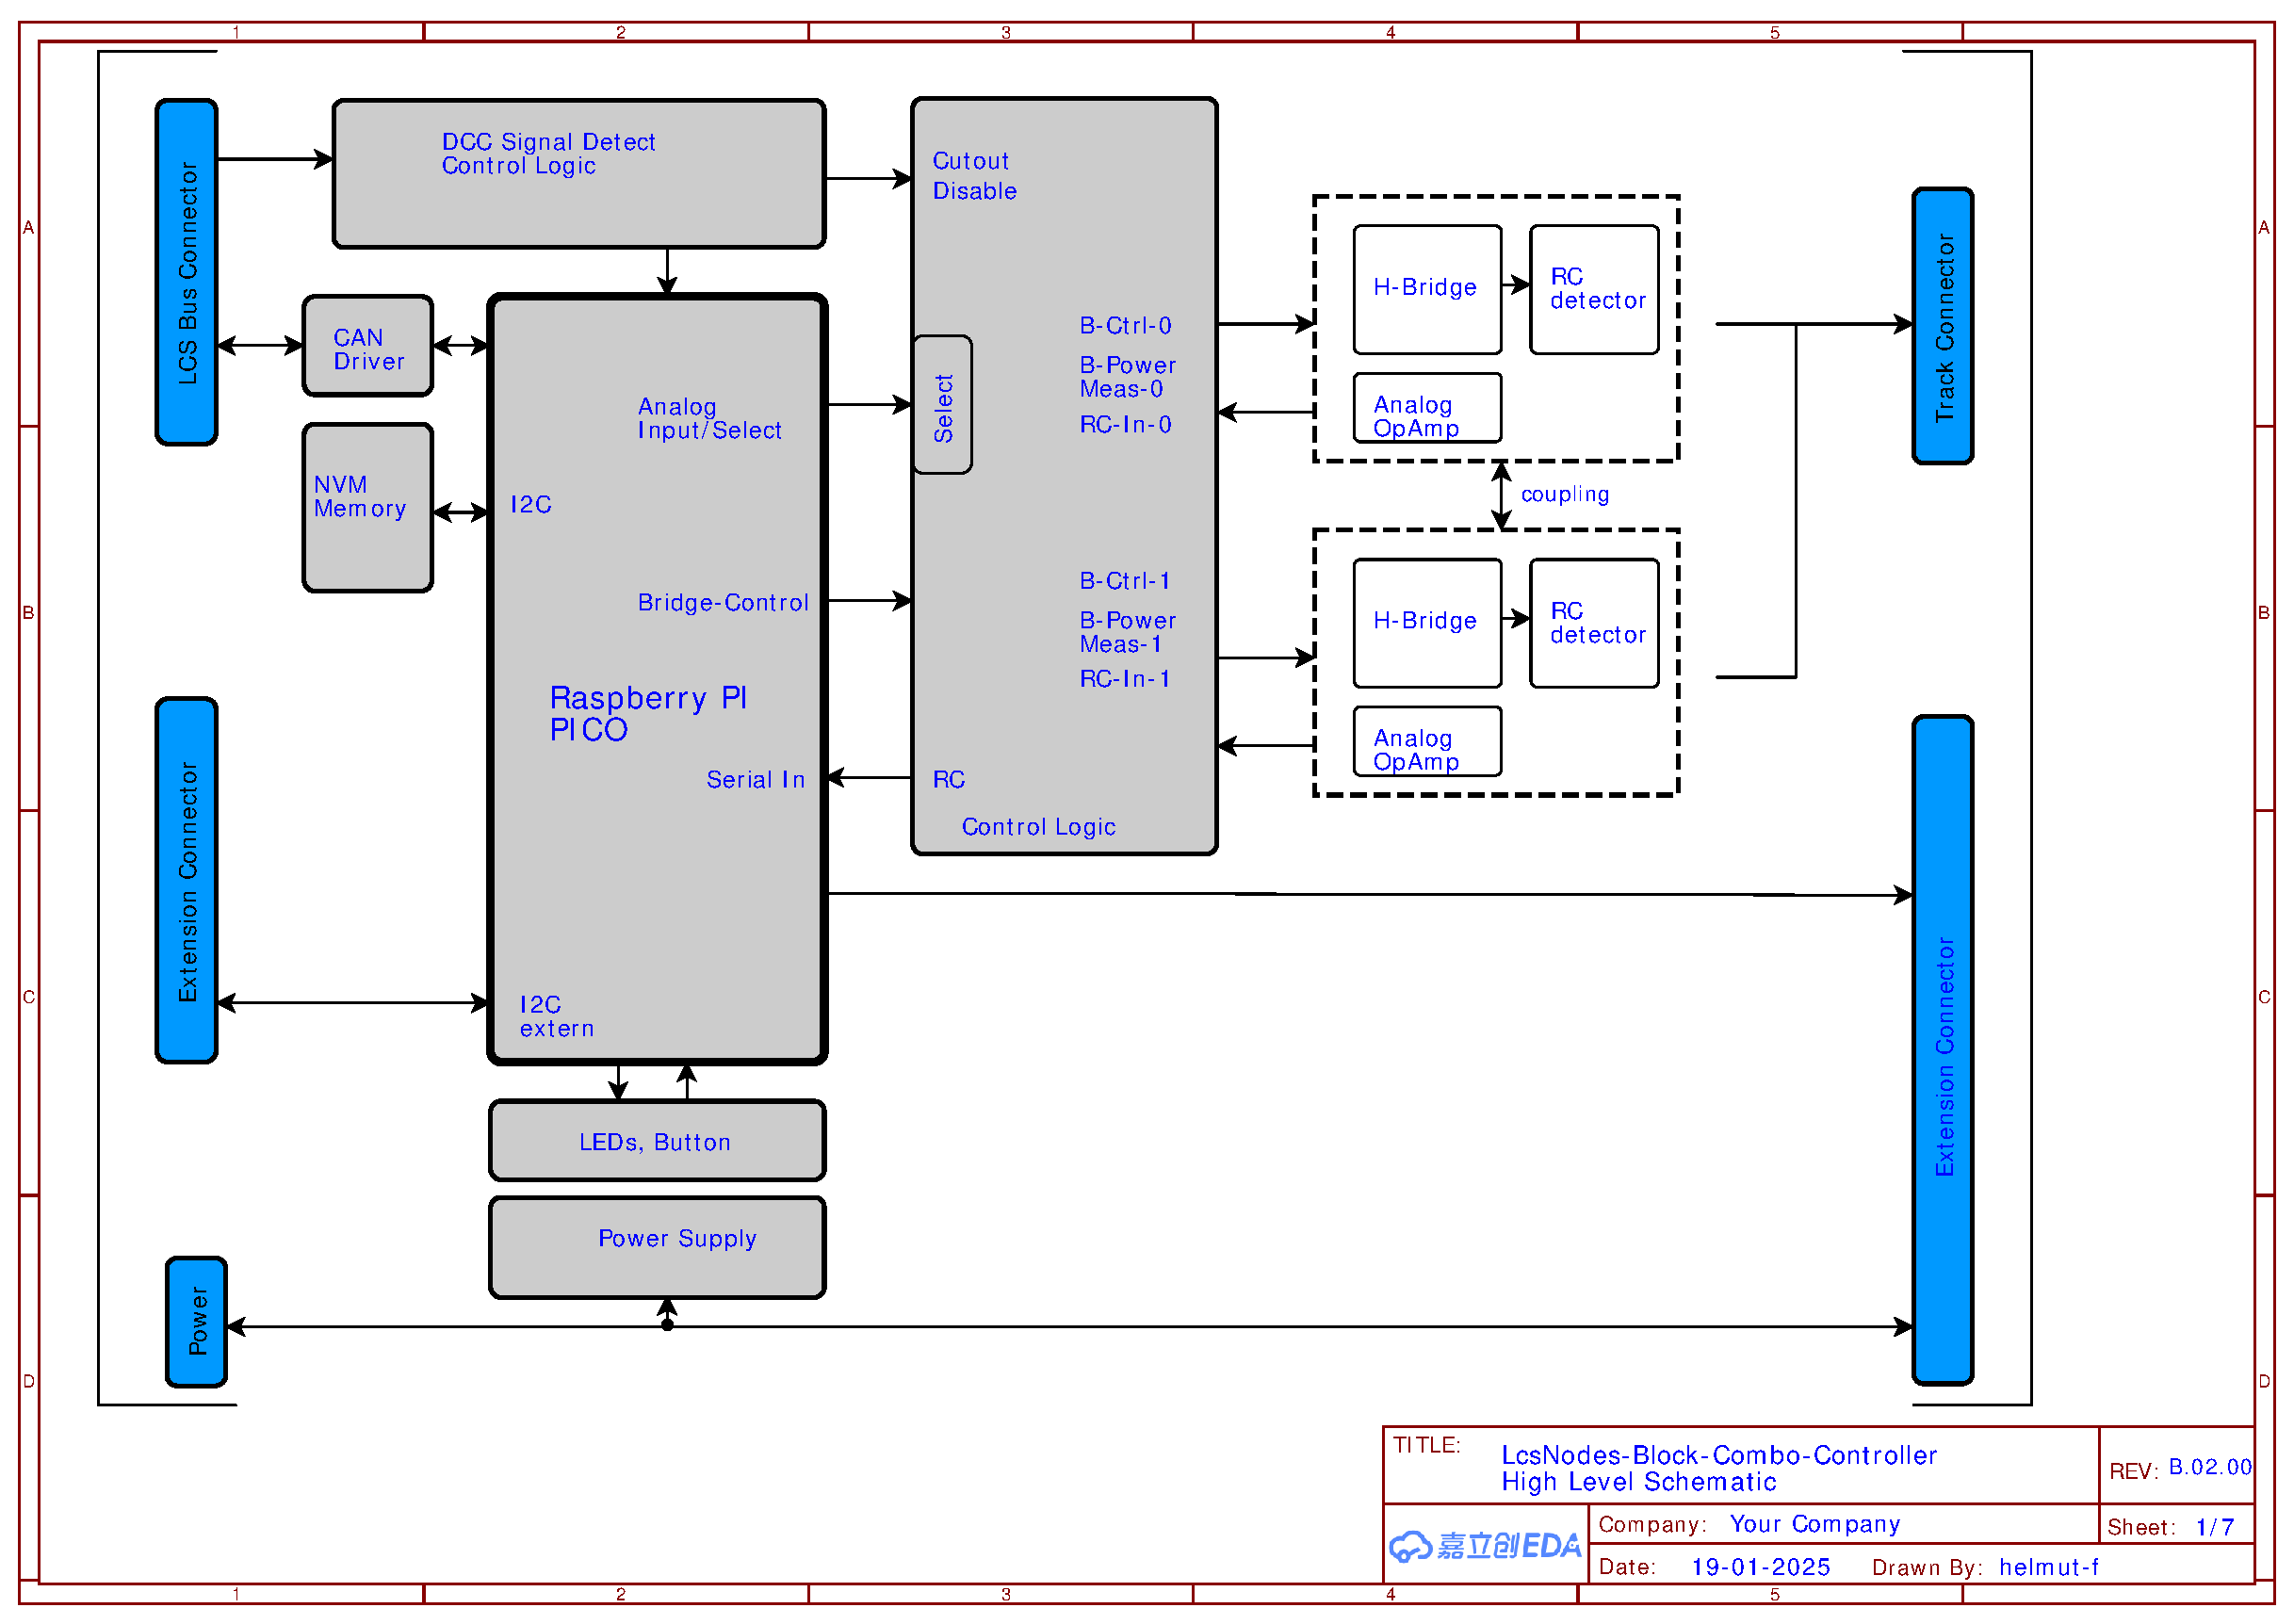
\includegraphics[page=1, width=0.7\textwidth]{./Schematics/Schematic_LcsNodes-Block-Combo-Controller.pdf}
    %\label{fig:schematic}
\end{figure}
\FloatBarrier

The main controller and the DCC signal decoding logic are identical to the quad controller.

\begin{figure}[htbp]
    \centering
    \includegraphics[page=2, width=0.7\textwidth]{./Schematics/Schematic_LcsNodes-Block-Combo-Controller.pdf}
    %\label{fig:schematic}
\end{figure}
\FloatBarrier

\begin{figure}[htbp]
    \centering
    \includegraphics[page=3, width=0.7\textwidth]{./Schematics/Schematic_LcsNodes-Block-Combo-Controller.pdf}
    %\label{fig:schematic}
\end{figure}
\FloatBarrier

The Dual H-Bridge control logic implements the same logic, however since there are only two channels, the enable logic is implemented slightly different. There is also a set of jumpers that will put the two H-Bridges in parallel mode. When the H-bridge is configured to run in that mode, the outputs are connected in parallel. The control logic is that of channel zero.

\begin{figure}[htbp]
    \centering
    \includegraphics[page=4, width=0.7\textwidth]{./Schematics/Schematic_LcsNodes-Block-Combo-Controller.pdf}
    %\label{fig:schematic}
\end{figure}
\FloatBarrier

The rest of the schematic is straightforward and other than we only need two instead of four units of RailCom, current amplifier and connectors is largely identical. Since we only have two current measurement units, there is no need to multiplex the analog signal. 

\begin{figure}[htbp]
    \centering
    \includegraphics[page=5, width=0.7\textwidth]{./Schematics/Schematic_LcsNodes-Block-Combo-Controller.pdf}
    %\label{fig:schematic}
\end{figure}
\FloatBarrier

\begin{figure}[htbp]
    \centering
    \includegraphics[page=6, width=0.7\textwidth]{./Schematics/Schematic_LcsNodes-Block-Combo-Controller.pdf}
    %\label{fig:schematic}
\end{figure}
\FloatBarrier

\begin{figure}[htbp]
    \centering
    \includegraphics[page=7, width=0.7\textwidth]{./Schematics/Schematic_LcsNodes-Block-Combo-Controller.pdf}
    %\label{fig:schematic}
\end{figure}
\FloatBarrier

\section{Summary}

Well, the design of the quad block controller, although simple in the individual components, was a champions league effort when it came to the PCB board design. It is the most complex board of all the board described in this book. The Combo block controller shows that with little effort and the right H-Bridge chip, a mono block controller with twice the amperage and a dual block controller can nicely be combined. We also abstracted the control of the power unit. From a firmware perspective, the bridge is controlled with two bits, putting the bridge in disconnected mode, PWM modes forward and reverse and finally DCC mode.

